\documentclass[a4paper]{article}
\usepackage{geometry}
\usepackage{graphicx}
\usepackage{natbib}
\usepackage{amsmath}
\usepackage{amssymb}
\usepackage{amsthm}
\usepackage{paralist}
\usepackage{epstopdf}
\usepackage{tabularx}
\usepackage{longtable}
\usepackage{multirow}
\usepackage{multicol}
\usepackage[hidelinks]{hyperref}
\usepackage{fancyvrb}
\usepackage{algorithm}
\usepackage{algorithmic}
\usepackage{float}
\usepackage{paralist}
\usepackage{parskip}
\usepackage[svgname]{xcolor}
\usepackage{enumerate}
\usepackage{array}
\usepackage{times}
\usepackage{url}
\usepackage{fancyhdr}
\usepackage{comment}
\usepackage{environ}
\usepackage{times}
\usepackage{textcomp}
\usepackage{caption}
\usepackage{color}
\usepackage{xcolor}
\usepackage{listings}
\usepackage{hyperref}
\usepackage{subcaption}

\urlstyle{rm}

\setlength\parindent{0pt} % Removes all indentation from paragraphs
\theoremstyle{definition}
\newtheorem{definition}{Definition}[]
\newtheorem{conjecture}{Conjecture}[]
\newtheorem{example}{Example}[]
\newtheorem{theorem}{Theorem}[]
\newtheorem{lemma}{Lemma}
\newtheorem{proposition}{Proposition}
\newtheorem{corollary}{Corollary}

\floatname{algorithm}{Procedure}
\renewcommand{\algorithmicrequire}{\textbf{Input:}}
\renewcommand{\algorithmicensure}{\textbf{Output:}}
\newcommand{\abs}[1]{\lvert#1\rvert}
\newcommand{\norm}[1]{\lVert#1\rVert}
\newcommand{\RR}{\mathbb{R}}
\newcommand{\CC}{\mathbb{C}}
\newcommand{\Nat}{\mathbb{N}}
\newcommand{\br}[1]{\{#1\}}
\DeclareMathOperator*{\argmin}{arg\,min}
\DeclareMathOperator*{\argmax}{arg\,max}
\renewcommand{\qedsymbol}{$\blacksquare$}

\definecolor{dkgreen}{rgb}{0,0.6,0}
\definecolor{gray}{rgb}{0.5,0.5,0.5}
\definecolor{mauve}{rgb}{0.58,0,0.82}

\newcommand{\Var}{\mathrm{Var}}
\newcommand{\Cov}{\mathrm{Cov}}

\newcommand{\vc}[1]{\boldsymbol{#1}}
\newcommand{\xv}{\vc{x}}
\newcommand{\Sigmav}{\vc{\Sigma}}
\newcommand{\alphav}{\vc{\alpha}}
\newcommand{\muv}{\vc{\mu}}

\newcommand{\red}[1]{\textcolor{red}{#1}}

\def\x{\mathbf x}
\def\y{\mathbf y}
\def\w{\mathbf w}
\def\v{\mathbf v}
\def\E{\mathbb E}
\def\V{\mathbb V}

% TO SHOW SOLUTIONS, include following (else comment out):
\newenvironment{soln}{
    \leavevmode\color{blue}\ignorespaces
}{}


\hypersetup{
%    colorlinks,
    linkcolor={red!50!black},
    citecolor={blue!50!black},
    urlcolor={blue!80!black}
}

\geometry{
  top=1in,            % <-- you want to adjust this
  inner=1in,
  outer=1in,
  bottom=1in,
  headheight=3em,       % <-- and this
  headsep=2em,          % <-- and this
  footskip=3em,
}


\pagestyle{fancyplain}
\lhead{\fancyplain{}{Homework 2}}
\rhead{\fancyplain{}{CS 760 Machine Learning}}
\cfoot{\thepage}

\title{\textsc{Homework 2}} % Title

%%% NOTE:  Replace 'NAME HERE' etc., and delete any "\red{}" wrappers (so it won't show up as red)

\author{
\red{APOORVA KUMAR} \\
\red{908 461 5997}\\
} 

\date{}

\begin{document}

\maketitle 


\textbf{Instructions:} 
Use this latex file as a template to develop your homework. Submit your homework on time as a single pdf file to Canvas. Please wrap your code and upload to a public GitHub repo, then attach the link below the instructions so that we can access it. You can choose any programming language (i.e. python, R, or MATLAB), as long as you implement the algorithm from scratch (e.g. do not use sklearn on questions 1 to 7 in section 2). Please check Piazza for updates about the homework.\\

\begin{soln}
    \Large
    \href{https://github.com/cybr17crwlr/ECE-760-Machine-Learning-Assignments/tree/master/Homework%202}{Homework 2 Github Link}
\end{soln}


\section{A Simplified Decision Tree}
You are to implement a decision-tree learner for classification.
To simplify your work, this will not be a general purpose decision tree.  Instead, your program can assume that
\begin{itemize}
\item each item has two continuous features $\x \in \RR^2$
\item the class label is binary and encoded as $y \in \{0,1\}$
\item data files are in plaintext with one labeled item per line, separated by whitespace:
$$x_{11} \quad x_{12} \quad y_1$$
$$...$$
$$x_{n1} \quad x_{n2} \quad y_n$$
\end{itemize}

Your program should implement a decision tree learner according to the following guidelines:
\begin{itemize}
\item Candidate splits $(j,c)$ for numeric features should use a threshold $c$ in feature dimension $j$ in the form of $x_{\cdot j}\ge c$.
\item $c$ should be on values of that dimension present in the training data; i.e. the threshold is on training points, not in between training points. You may enumerate all features, and for each feature, use all possible values for that dimension.
\item You may skip those candidate splits with zero split information (i.e. the entropy of the split), and continue the enumeration.
\item The left branch of such a split is the ``then'' branch, and the right branch is ``else''.
\item Splits should be chosen using information gain ratio. If there is a tie you may break it arbitrarily.
\item The stopping criteria (for making a node into a leaf) are that 
	\begin{itemize}
	\item the node is empty, or
	\item all splits have zero gain ratio (if the entropy of the split is non-zero), or
	\item the entropy of any candidates split is zero
	\end{itemize}
\item To simplify, whenever there is no majority class in a leaf, let it predict $y=1$.
\end{itemize}

\section{Questions}
\begin{enumerate}
\item (Our algorithm stops at pure labels) [10 pts] If a node is not empty but contains training items with the same label, why is it guaranteed to become a leaf?  Explain. You may assume that the feature values of these items are not all the same.\\
\begin{soln}
    When a node has pure labels the Information gain from that node $H(X)-H(X/S)$ becomes zero for any \textit{Candidate Split $S$} and thus splitting here helps the algorithm is no way and it becomes a leaf node.
\end{soln}

\item (Our algorithm is greedy)  [10 pts] Handcraft a small training set where both classes are present but the algorithm refuses to split; instead it makes the root a leaf and stop;
Importantly, if we were to manually force a split, the algorithm will happily continue splitting the data set further and produce a deeper tree with zero training error.
You should (1) plot your training set, (2) explain why.  Hint: you don't need more than a handful of items. \\
\begin{soln}
    Lets choose the following dataset:\\
    \begin{minipage}{0.4\linewidth}
        \begin{figure}[H]
            \centering
            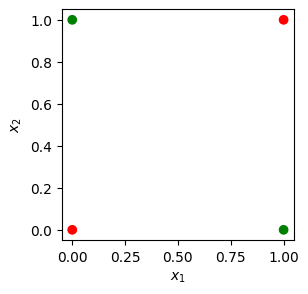
\includegraphics[scale=0.5]{Images/Q2/DTq2.png}
            \label{fig:q2}
        \end{figure}
    \end{minipage}
    \begin{minipage}{0.3\linewidth}
        \centering
        \large
        \begin{tabular}{|c|c|c|}
            \hline
            $x_1$ & $x_2$ & label \\
            \hline
            0 & 0 & 0 \\
            0 & 1 & 1 \\
            1 & 0 & 1 \\
            1 & 1 & 0 \\
            \hline
        \end{tabular}
    \end{minipage}
    \begin{minipage}{0.3\linewidth}
        Splitting $x_1\geq c$, $c\in\{0,1\}$\\\\
        $x_1 < 1$\\
        \begin{tabular}{|c|c|c|}
            \hline
            $x_1$ & $x_2$ & label \\
            \hline
            0 & 0 & 0 \\
            0 & 1 & 1 \\
            \hline
        \end{tabular}\\

        
        $x_1\geq 1$\\
        \begin{tabular}{|c|c|c|}
            \hline
            $x_1$ & $x_2$ & label \\
            \hline
            1 & 0 & 1 \\
            1 & 1 & 0 \\
            \hline
        \end{tabular}
    \end{minipage}\\
    Now we know our algorithm splits using a linear boundary along one of the dimensions. Thus for our dataset, any linear boundary results is zero information gain.\\ Lets split along a point $c \in \{0,1\}$ such that $x_1 \geq c$
    \begin{gather*}
        H(x_1,x_2) = 1/2\log{2}+1/2\log{2} = \log{2}\\
        H(x_1,x_2/x_1\geq c) = 1/2(1/2\log{2}+1/2\log{2}) + 1/2(1/2\log{2}+1/2\log{2}) = \log{2}\\
        \text{Info Gain} = H(x_1,x_2) - H(x_1,x_2/x_1\geq c) = 0
    \end{gather*}\\
   The same can be shown for $x_2$ as the dataset is symmetric. This eventually means that we end up in a situation, such as the above example, for a dataset without a single linear boundary and no correlation between the variables.

    It's also easy to note that if we force a split, then in the later stages, the algorithm with continue splitting as it gets a positive information gain boundary after any forced split. For example, in the above split, we can see that each node can now be split easily using $x_2$ to produce a tree with zero error.
\end{soln}

\item (Information gain ratio exercise)  [10 pts] Use the training set \texttt{Druns.txt}.  For the root node, list all candidate cuts and their information gain ratio. If the entropy of the candidate split is zero, please list its mutual information (i.e. information gain). Hint: to get $\log_2(x)$ when your programming language may be using a different base, use \verb|log(x)/log(2)|. Also, please follow the split rule in the first section. \\
\begin{soln}
    \begin{tabular}{|c|c|c|c|}
        \hline
        \textbf{Feature} & \textbf{Cutoff} & \textbf{Info. Gain Ratio} & \textbf{Info. Gain} \\
        \hline
        \textit{X1} & \textit{0.0} & -- & \textit{0.0} \\
        X1 & 0.1 & 0.10051807676021828 & -- \\
        \hline
        \textit{X2} & \textit{-2.0} & -- & \textit{0.0} \\
        X2 & -1.0 & 0.10051807676021828 & -- \\
        X2 & 0.0 & 0.05595375963126383 & -- \\
        X2 & 1.0 & 0.005780042205152189 & -- \\
        X2 & 2.0 & 0.001144349517276632 & -- \\
        X2 & 3.0 & 0.016411136842102023 & -- \\
        X2 & 4.0 & 0.049749064181778435 & -- \\
        X2 & 5.0 & 0.11124029586339801 & -- \\
        X2 & 6.0 & 0.236099606143608 & -- \\
        X2 & 7.0 & 0.05595375963126383 & -- \\
        X2 & 8.0 & 0.4301569161309807 & -- \\
        \hline
    \end{tabular}
\end{soln}

\item (The king of interpretability)  [10 pts] Decision tree is not the most accurate classifier in general.  However, it persists.  This is largely due to its rumored interpretability: a data scientist can easily explain a tree to a non-data scientist.  Build a tree from D3leaves.txt.  Then manually convert your tree to a set of logic rules.  Show the tree\footnote{When we say show the tree, we mean either the standard computer science tree view, or some crude plaintext representation of the tree -- as long as you explain the format.  When we say visualize the tree, we mean a plot in the 2D $\x$ space that shows how the tree will classify any points.} and the rules. \\

\begin{soln}
    \begin{minipage}{0.5\linewidth}
        The tree built by the logic is:
        \begin{lstlisting}
        {
          "X1": {
            ">=10 then": 1,
            "else <10": {
              "X2": {
                ">=3 then": 1,
                "else <3": 0
              }
            }
          }
        }
        \end{lstlisting}
    \end{minipage}
    \begin{minipage}{0.5\linewidth}
        Logically this means the following:
        \begin{figure}[H]
            \centering
            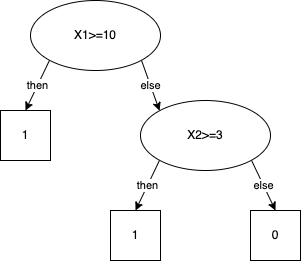
\includegraphics[scale=0.5]{Images/Q4/DTq4.png}
            \label{fig:q4}
        \end{figure}
    \end{minipage}
    
\end{soln}

\item (Or is it?)  [20 pts] For this question only, make sure you DO NOT VISUALIZE the data sets or plot your tree's decision boundary in the 2D $\x$ space.  If your code does that, turn it off before proceeding.  This is because you want to see your own reaction when trying to interpret a tree.  You will get points no matter what your interpretation is.
And we will ask you to visualize them in the next question anyway.
  \begin{itemize}
  
  \item Build a decision tree on D1.txt.  Show it to us in any format (e.g. could be a standard binary tree with nodes and arrows, and denote the rule at each leaf node; or as simple as plaintext output where each line represents a node with appropriate line number pointers to child nodes; whatever is convenient for you). Again, do not visualize the data set or the tree in the $\x$ input space.  In real tasks you will not be able to visualize the whole high dimensional input space anyway, so we don't want you to ``cheat'' here.
  \begin{soln}
      The tree built by the logic is:
        \begin{lstlisting}
        {
          "X2": {
            ">=0.201829 then": 1,
            "else <0.201829": 0
          }
        }
        \end{lstlisting}
  \end{soln}
  
  \item Look at your tree in the above format (remember, you should not visualize the 2D dataset or your tree's decision boundary) and try to interpret the decision boundary in human understandable English. 
  \begin{soln}
      The above logic means if \textbf{$\mathbf{X_2\geq0.201829}$ then} classify the datapoint \textit{in class 1}, \textbf{else} classify it \textit{in class 0}
  \end{soln}
  
  \item Build a decision tree on D2.txt.  Show it to us.
  \begin{soln}
      \begin{lstlisting}
          {
          "X1": {
            ">=0.533076 then": {
              "X2": {
                ">=0.228007 then": {
                  "X2": {
                    ">=0.424906 then": 1,
                    "else <0.424906": {
                      "X1": {
                        ">=0.708127 then": 1,
                        "else <0.708127": {
                          "X2": {
                            ">=0.32625 then": {
                              "X1": {
                                ">=0.595471 then": {
                                  "X1": {
                                    ">=0.646007 then": 1,
                                    "else <0.646007": {
                                      "X2": {
                                        ">=0.403494 then": 1,
                                        "else <0.403494": 0
                                      }
                                    }
                                  }
                                },
                                "else <0.595471": 0
                              }
                            },
                            "else <0.32625": 0
                          }
                        }
                      }
                    }
                  }
                },
                "else <0.228007": {
                  "X1": {
                    ">=0.887224 then": {
                      "X2": {
                        ">=0.037708 then": {
                          "X2": {
                            ">=0.082895 then": 1,
                            "else <0.082895": {
                              "X1": {
                                ">=0.960783 then": 1,
                                "else <0.960783": 0
                              }
                            }
                          }
                        },
                        "else <0.037708": 0
                      }
                    },
                    "else <0.887224": {
                      "X1": {
                        ">=0.850316 then": {
                          "X2": {
                            ">=0.169053 then": 1,
                            "else <0.169053": 0
                          }
                        },
                        "else <0.850316": 0
                      }
                    }
                  }
                }
              }
            },
            "else <0.533076": {
              "X2": {
                ">=0.88635 then": {
                  "X1": {
                    ">=0.041245 then": {
                      "X1": {
                        ">=0.104043 then": 1,
                        "else <0.104043": {
                          "X1": {
                            ">=0.07642 then": 0,
                            "else <0.07642": 1
                          }
                        }
                      }
                    },
                    "else <0.041245": 0
                  }
                },
                "else <0.88635": {
                  "X2": {
                    ">=0.691474 then": {
                      "X1": {
                        ">=0.254049 then": 1,
                        "else <0.254049": {
                          "X1": {
                            ">=0.191915 then": {
                              "X2": {
                                ">=0.792752 then": 1,
                                "else <0.792752": 0
                              }
                            },
                            "else <0.191915": {
                              "X2": {
                                ">=0.864128 then": {
                                  "X1": {
                                    ">=0.144781 then": 1,
                                    "else <0.144781": 0
                                  }
                                },
                                "else <0.864128": 0
                              }
                            }
                          }
                        }
                      }
                    },
                    "else <0.691474": {
                      "X2": {
                        ">=0.534979 then": {
                          "X1": {
                            ">=0.426073 then": 1,
                            "else <0.426073": {
                              "X1": {
                                ">=0.409972 then": {
                                  "X1": {
                                    ">=0.417579 then": 0,
                                    "else <0.417579": 1
                                  }
                                },
                                "else <0.409972": {
                                  "X1": {
                                    ">=0.393227 then": {
                                      "X1": {
                                        ">=0.39583 then": 0,
                                        "else <0.39583": 1
                                      }
                                    },
                                    "else <0.393227": 0
                                  }
                                }
                              }
                            }
                          }
                        },
                        "else <0.534979": 0
                      }
                    }
                  }
                }
              }
            }
          }
        }
      \end{lstlisting}
  \end{soln}
  
  \item Try to interpret your D2 decision tree. Is it easy or possible to do so without visualization? \\
  \begin{soln}
      Its not easy to interpret this solution without any plotting as it gets harder to track back up after reaching a leaf node in such a drastically split tree.
  \end{soln}
  
  \end{itemize}

\item (Hypothesis space)  [10 pts] For D1.txt and D2.txt, do the following separately:
  \begin{itemize}
  
  \item Produce a scatter plot of the data set.\\
    \begin{soln}
        For \texttt{D1.txt} the dataset looks like follows:
        \begin{figure}[H]
            \begin{subfigure}{0.5\textwidth}
                \centering
                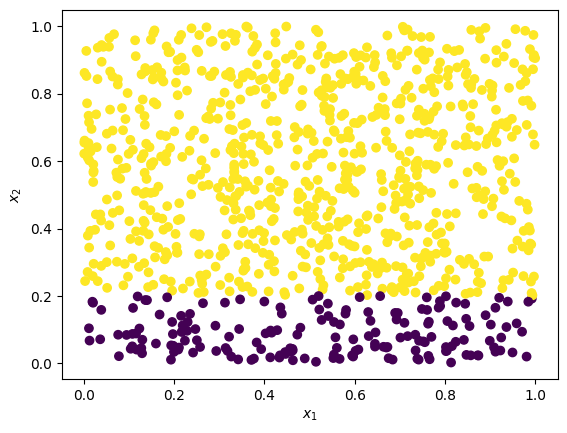
\includegraphics[scale=0.3]{Images/Q6/DTq6d1.png}
            \end{subfigure}%
            \begin{subfigure}{0.5\textwidth}
                \centering
                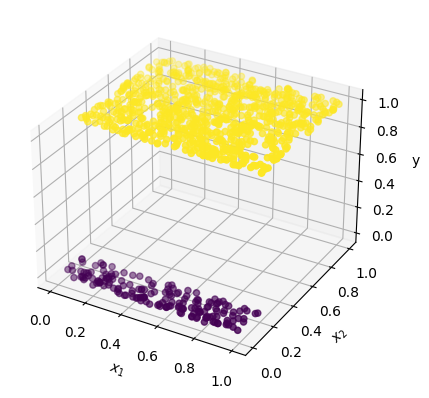
\includegraphics[scale=0.3]{Images/Q6/DTq6d1_3d.png}
            \end{subfigure}
            \label{fig:q6_d1}
        \end{figure}
        
        For \texttt{D2.txt} the dataset looks like follows:
        \begin{figure}[H]
            \begin{subfigure}{0.5\textwidth}
                \centering
                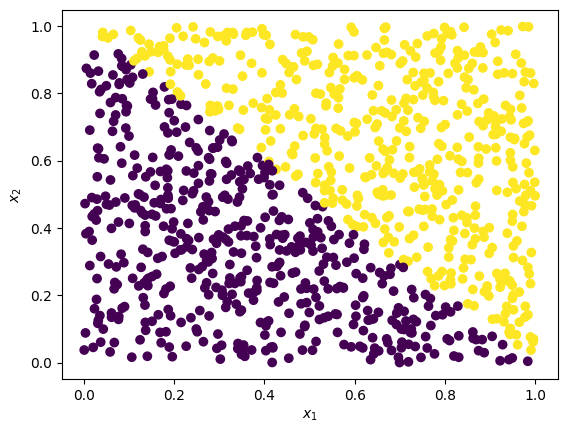
\includegraphics[scale=0.3]{Images/Q6/DTq6d2.png}
            \end{subfigure}%
            \begin{subfigure}{0.5\textwidth}
                \centering
                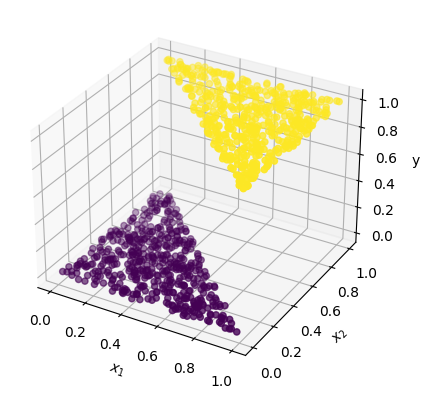
\includegraphics[scale=0.3]{Images/Q6/DTq6d2_3d.png}
            \end{subfigure}
            \label{fig:q6_d2}
        \end{figure}
    \end{soln}
  \item Visualize your decision tree's decision boundary (or decision region, or some other ways to clearly visualize how your decision tree will make decisions in the feature space).\\
  \begin{soln}
      For \texttt{D1.txt} the decision boundary looks like follows:
        \begin{figure}[H]
            \begin{subfigure}{0.5\textwidth}
                \centering
                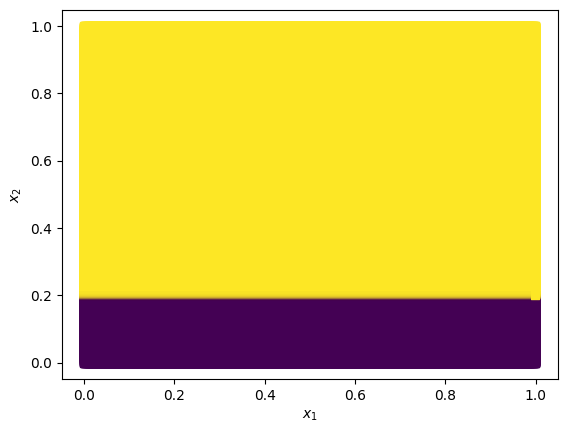
\includegraphics[scale=0.3]{Images/Q6/DTq6d1_bound.png}
            \end{subfigure}%
            \begin{subfigure}{0.5\textwidth}
                \centering
                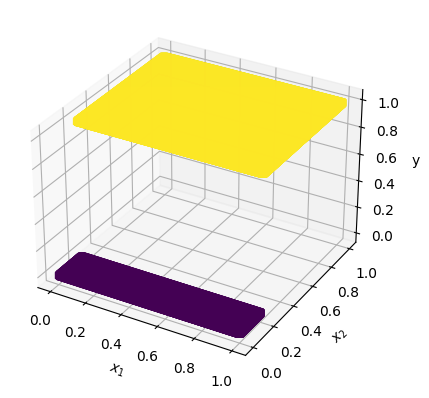
\includegraphics[scale=0.3]{Images/Q6/DTq6d1_bound_3d.png}
            \end{subfigure}
            \label{fig:q6_d1_bound}
        \end{figure}
      For \texttt{D2.txt} the decision boundary looks like follows:
        \begin{figure}[H]
            \begin{subfigure}{0.5\textwidth}
                \centering
                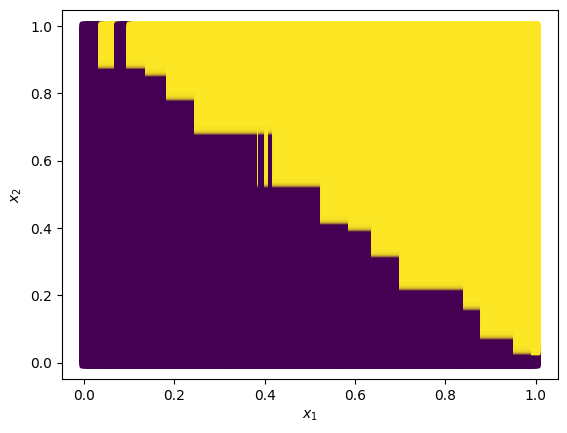
\includegraphics[scale=0.3]{Images/Q6/DTq6d2_bound.png}
            \end{subfigure}%
            \begin{subfigure}{0.5\textwidth}
                \centering
                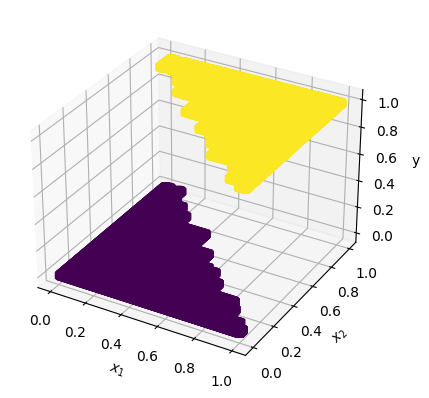
\includegraphics[scale=0.3]{Images/Q6/DTq6d2_bound_3d.png}
            \end{subfigure}
            \label{fig:q6_d2_bound}
        \end{figure}
  \end{soln}

  \end{itemize}
Then discuss why the size of your decision trees on D1 and D2 differ.  Relate this to the hypothesis space of our decision tree algorithm. \\
\begin{soln}
    As stated before, our proposed algorithm draws decision lines parallel to either axis and splits the data according to that. Due to this property of our Decision Tree, it can't learn any correlation between its feature variables and use the same to create a division in the hypothesis space. We can see its implications in the two different datasets we have. \texttt{D1.txt} has a hypothesis space separation along a single dimension, i.e., $x_2$, and thus we get a perfect decision boundary. On the other hand, for \texttt{D2.txt}, we have the decision boundary like $x_2+x_1=1$. Our algorithm cannot formulate such a hypothesis space separation. Thus the model tries to do a makeshift stair-like separator with boundaries parallel to either axis. 
\end{soln}

\item (Learning curve)  [20 pts] We provide a data set \texttt{Dbig.txt} with 10000 labeled items.  Caution: \texttt{Dbig.txt} is sorted.
  \begin{itemize}
  
  \item You will randomly split \texttt{Dbig.txt} into a candidate training set of 8192 items and a test set (the rest).  Do this by generating a random permutation, and split at 8192.
  
  \item Generate a sequence of five nested training sets $D_{32} \subset D_{128} \subset D_{512} \subset D_{2048} \subset D_{8192}$ from the candidate training set.  The subscript $n$ in $D_n$ denotes training set size.  The easiest way is to take the first $n$ items from the (same) permutation above.  This sequence simulates the real world situation where you obtain more and more training data.
  
  \item For each $D_n$ above, train a decision tree.  Measure its test set error $err_n$.  Show three things in your answer: (1) List $n$, number of nodes in that tree, $err_n$. (2) Plot $n$ vs. $err_n$.  This is known as a learning curve (a single plot). (3) Visualize your decision trees' decision boundary (five plots). \\
  
  \begin{soln}
    \begin{minipage}{0.3\linewidth}
        \begin{tabular}{|c|c|c|}
              \hline
              $\mathbf{n}$ & \textbf{Nodes} & $\mathbf{err_n }$ (in \%) \\
              \hline
              32 & 4 & 16.37 \\
              128 & 14 & 9.07 \\
              512 & 29 & 5.25 \\
              2048 & 68 & 4.37 \\
              8192 & 126 & 1.99 \\
              \hline
          \end{tabular}
    \end{minipage}
    \begin{minipage}{0.7\linewidth}
        \begin{figure}[H]
            \centering
            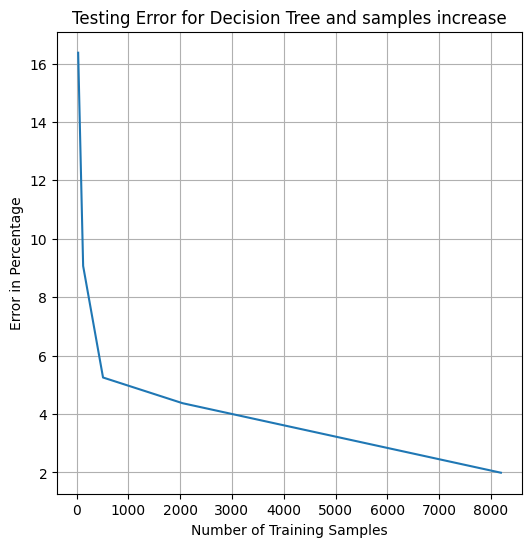
\includegraphics[scale=0.4]{Images/Q7/DTq7_error.png}
            \label{fig:q7_error}
        \end{figure}
    \end{minipage}

    Decision Boundary with training points are shown below:\\
    \begin{figure}[H]
        \begin{subfigure}{0.5\textwidth}
            \centering
            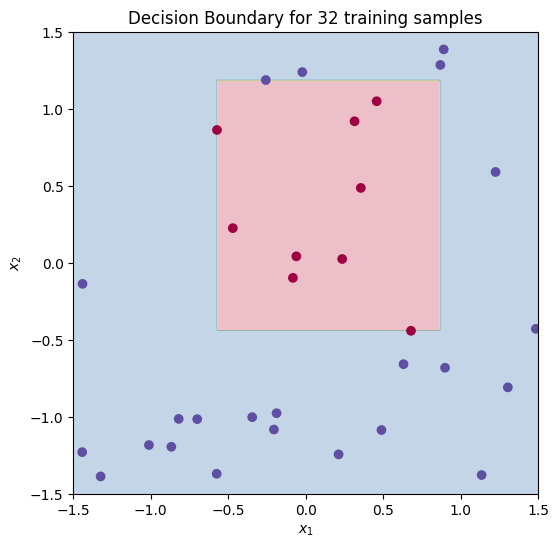
\includegraphics[scale=0.4]{Images/Q7/DTq7_32.png}
            \label{fig:q7_32}
        \end{subfigure}%
        \begin{subfigure}{0.5\textwidth}
            \centering
            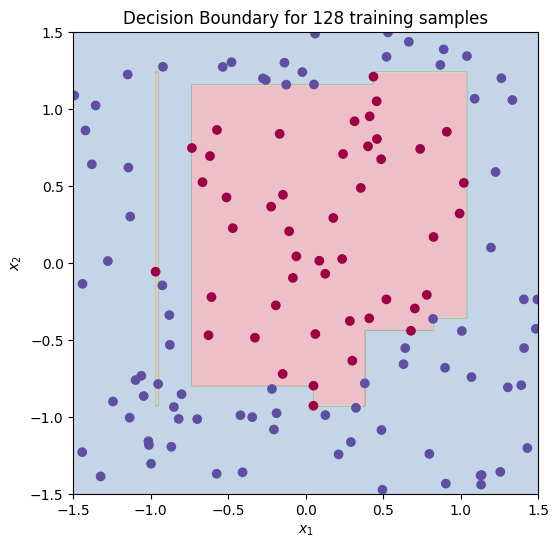
\includegraphics[scale=0.4]{Images/Q7/DTq7_128.png}
            \label{fig:q7_128}
        \end{subfigure}
    \end{figure}
    \begin{figure}[H]
        \begin{subfigure}{0.5\textwidth}
            \centering
            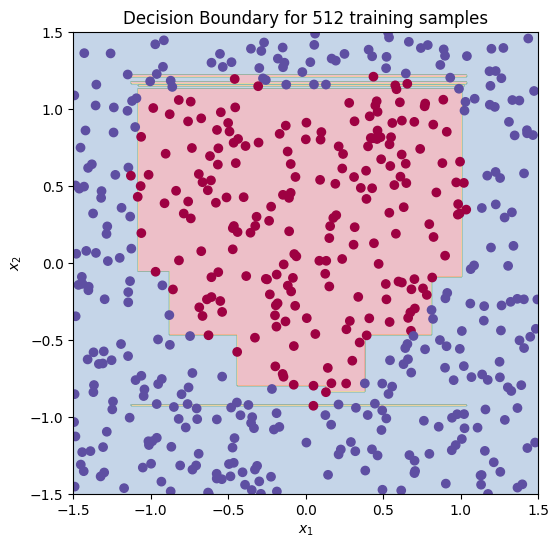
\includegraphics[scale=0.4]{Images/Q7/DTq7_512.png}
            \label{fig:q7_512}
        \end{subfigure}%
        \begin{subfigure}{0.5\textwidth}
            \centering
            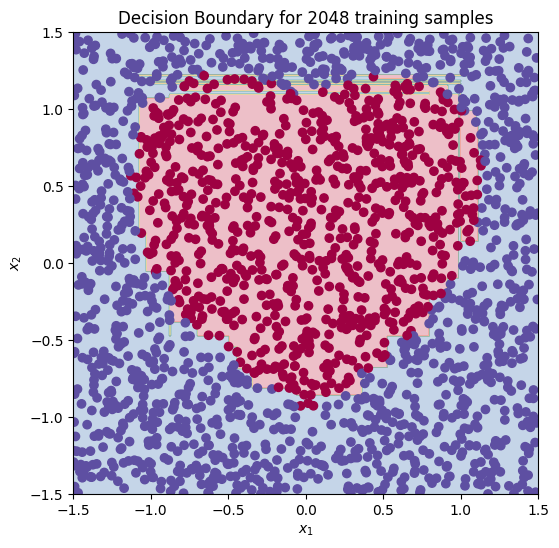
\includegraphics[scale=0.4]{Images/Q7/DTq7_2048.png}
            \label{fig:q7_2048}
        \end{subfigure}
    \end{figure}
    \begin{figure}[H]
        \centering
        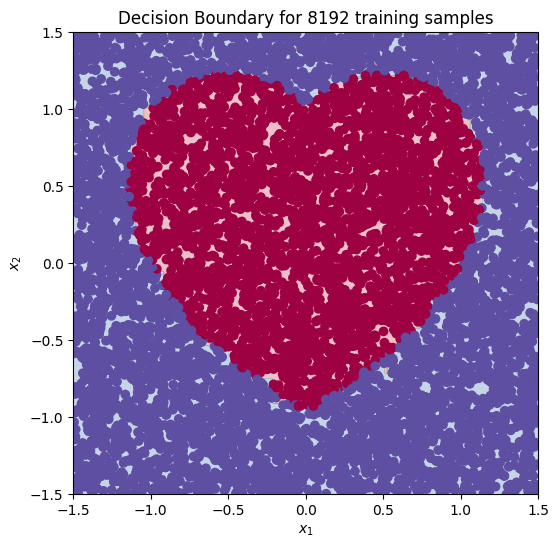
\includegraphics[scale=0.4]{Images/Q7/DTq7_8192.png}
        \label{fig:q7_8192}
    \end{figure}
    
  \end{soln}
  \end{itemize}
  
\end{enumerate}

\section{sklearn [10 pts]}
Learn to use sklearn (\url{https://scikit-learn.org/stable/}).
Use sklearn.tree.DecisionTreeClassifier to produce trees for datasets $D_{32}, D_{128}, D_{512}, D_{2048}, D_{8192}$.  Show two things in your answer: (1) List $n$, number of nodes in that tree, $err_n$. (2) Plot $n$ vs. $err_n$.

\begin{soln}
    Using the same seed as Question 7 we create the same split in data and notice the following result:\\
    \begin{minipage}{0.4\linewidth}
        \centering
        \begin{tabular}{|c|c|c|}
              \hline
              $\mathbf{n}$ & \textbf{Nodes} & $\mathbf{err_n }$ (in \%) \\
              \hline
              32 & 9 & 10.73 \\
              128 & 33 & 6.91 \\
              512 & 53 & 4.42 \\
              2048 & 107 & 3.43 \\
              8192 & 223 & 1.38 \\
              \hline
          \end{tabular}
    \end{minipage}
    \begin{minipage}{0.6\linewidth}
        \begin{figure}[H]
            \centering
            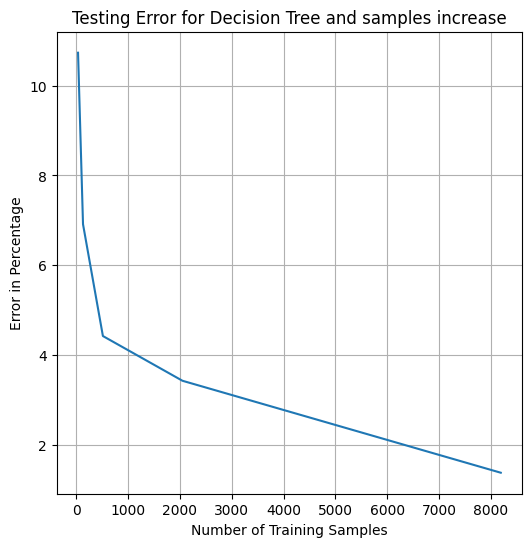
\includegraphics[scale=0.4]{Images/DTsk_error.png}
            \label{fig:qsk_error}
        \end{figure}
    \end{minipage}
\end{soln}

\section{Lagrange Interpolation [10 pts]}
Fix some interval $[a, b]$ and sample $n = 100$ points $x$ from this interval uniformly. Use these to build a training set consisting of $n$ pairs $(x, y)$ by setting function $y = sin(x)$. \\
\begin{soln}
    For a = 0 and b = $4\pi$. The training set of 100 points looks as follows:
    \begin{figure}[H]
        \centering
        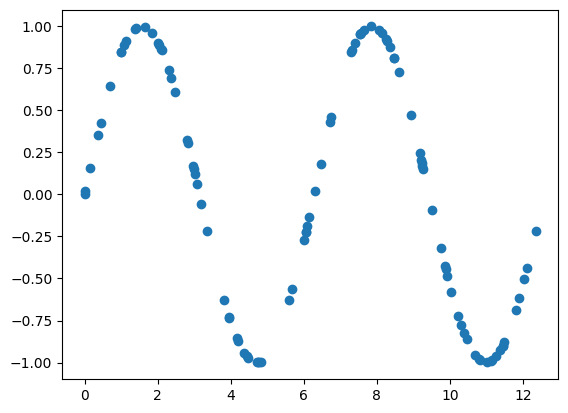
\includegraphics[scale=0.4]{Images/DTlang_train.png}
        \label{fig:lang_train}
    \end{figure}
    
\end{soln}

Build a model $f$ by using Lagrange interpolation, check more details in \url{https://en.wikipedia.org/wiki/Lagrange_polynomial} and \url{https://docs.scipy.org/doc/scipy/reference/generated/scipy.interpolate.lagrange.html}. \\

Generate a test set using the same distribution as your test set. Compute and report the resulting model’s train and test error. What do you observe?
Repeat the experiment with zero-mean Gaussian noise $\epsilon$ added to $x$. Vary the standard deviation for $\epsilon$ and report your findings.\\
\begin{soln}
    When training with the whole set of 100 points, I observed a higher error in interpolation estimation than training with a small set of points sampled randomly from the whole dataset. Hence, I will report the error when training with both cases.\\
    Note: When calculating the training error, it is calculated for only the training samples, i.e., for 100 samples, the error is for 100 points, and for like 17 points, its for 17 points.
    
    Below are the results for errors:\\
    \begin{center}
        \begin{tabular}{|c|c|c|c|c|c|}
            \hline
            \multirow{2}{6em}{\textbf{Model Name}} & \multirow{2}{4em}{\textbf{Std Dev.}} & \multicolumn{2}{c|}{\textbf{Training Error}} & \multicolumn{2}{c|}{\textbf{Testing Error}}\\
            & & 100 samples & 17 samples & 100 samples & 17 samples \\
            \hline
            Base Model & -- & 1.58e+79 & 0.00188 & 1.059e+79 & 0.00199 \\
            \multirow{6}{6em}{Model with Noise} & 0.001 & 1.84e+78 & 0.00175 & 2.52e+77 & 442.48 \\
             & 0.01 & 1.004e+78 & 0.00615 & 1.11e+77 & 110962.58 \\
             & 0.1 & 6.66e+78 & 0.254 & 5.38e+77 & 931810.65 \\
             & 1 & 2.69e+82 & 0.000111 & 2.55e+77 & 17260.72 \\
             & 10 & 6.96e+65 & 0.00106 & 9.17e+38 & 7748.92 \\
             & 100 & 2.33e+72 & 3.61e-07 & 9688736.27 & 137.51 \\
            \hline
        \end{tabular}
    \end{center}
    We can see that while the Training Error maintains itself the Testing error first rises then starts falling again as standard deviation of noise increases.
\end{soln}

\bibliographystyle{apalike}
\end{document}
